\subsection{傅里叶变换的性质}

\subsubsection{FT 是线性运算}

\begin{property}
    设 $f(t)$ 和 $g(t)$ 是两个信号,$a$ 和 $b$ 是两个常数,
    且 $F(\omega)$ 和 $G(\omega)$ 分别是 $f(t)$ 和 $g(t)$ 的 FT,
    则有
    \begin{align*}
        \mathcal{F}[af(t) + bg(t)] = aF(\omega) + bG(\omega).
    \end{align*}
    这说明,对一个信号求 FT,等于对其分量(分信号)求 FT 然后再组合。
\end{property}

\begin{remark}
    FT 是线性运算,是因为 FT 既有\bd{齐次性},又有\bd{叠加性}。
    齐次性是指 $\mathcal{F}[af(t)] = a\mathcal{F}[f(t)]$,
    叠加性是指 $\mathcal{F}[f(t) + g(t)] = \mathcal{F}[f(t)] + \mathcal{F}[g(t)]$。
\end{remark}

\subsubsection{FT 的反褶和共轭的性质}

\begin{property}
    设信号 $f(t)$ 的 FT 为 $F(\omega)$,则进行反褶和共轭操作后的信号的 FT 对应关系如下:
    \begin{figure}[H]
        \begin{tabular}
            {c||c|c}
            操作 & 时域 & 频域 \\
            \hline
            反褶 & $f(-t)$ & $F(-\omega)$ \\
            共轭 & $f^*(t)$ & $F^*(-\omega)$ \\
            反褶且共轭 & $f^*(-t)$ & $F^*(\omega)$ \\
        \end{tabular}
    \end{figure}
\end{property}

\subsubsection{傅里叶变换及其逆变换的对偶性}

注意到 FT 和 IFT 在形式上极为相似:
\begin{align*}
    F(\omega) & = \quad\;\; \int_{-\infty}^{+\infty} f(t)\mathe^{-\mathi\omega t}\D{t}, \\
    f(t) & = \frac{1}{2\pi} \int_{-\infty}^{+\infty} F(\omega)\mathe^{\mathi\omega t}\D{\omega}.
\end{align*}
所以,我们可以尝试从这个切入点入手,来研究 FT 和 IFT 之间的关系。

\begin{lemma}[FT 和 IFT 的变换核之间的关系]
    FT 与 IFT 的变换核函数是共轭对称的,即
    \begin{align*}
        (\mathe^{-\mathi\omega t})^* = \mathe^{\mathi\omega t}, \quad
        (\mathe^{\mathi\omega t})^* = \mathe^{-\mathi\omega t}.
    \end{align*}
\end{lemma}

\begin{proof}
    由共轭的定义,我们有
    \begin{align*}
        (\mathe^{-\mathi\omega t})^* = (\cos\omega t - \mathi\sin\omega t)^* = \cos\omega t + \mathi\sin\omega t = \mathe^{\mathi\omega t}, \\
        (\mathe^{\mathi\omega t})^* = (\cos\omega t + \mathi\sin\omega t)^* = \cos\omega t - \mathi\sin\omega t = \mathe^{-\mathi\omega t}.
    \end{align*}
    命题得证。
\end{proof}

这说明,FT 和 IFT 的变换核之间是共轭对称的。因此,IFT 可以由 FT 来完成:

\begin{theorem}
    设 $f(t)$ 是一个信号,其 FT 为 $F(\omega)$,则有
    \begin{align*}
        \mathcal{F}^{-1}[F(\omega)] = f(t) = \frac{1}{2\pi}\{\mathcal{F}_{\omega}[F^*(\omega)]\}^*.
    \end{align*}
    其中 $\mathcal{F}_\omega(\cdot)$ 表示以 $\omega$ 为自变量求 FT,结果为 $t$ 的函数。
\end{theorem}

\begin{proof}
    根据 IFT 的定义,我们有
    \begin{align*}
        f(t) = \frac{1}{2\pi} \int_{-\infty}^{+\infty} F(\omega)\mathe^{\mathi\omega t}\D{\omega}.
    \end{align*}
    由于 FT 和 IFT 的变换核之间是共轭对称的,我们有
    \begin{align*}
        f(t) & = \frac{1}{2\pi} \int_{-\infty}^{+\infty} F(\omega)\mathe^{\mathi\omega t}\D{\omega} \\
        & = \frac{1}{2\pi} \int_{-\infty}^{+\infty} F(\omega)(\mathe^{-\mathi\omega t})^*\D{\omega} \\
        & = \frac{1}{2\pi} \left\{\int_{-\infty}^{+\infty} F^*(\omega)\mathe^{-\mathi\omega t}\D{\omega}\right\}^* \\
        & = \frac{1}{2\pi}\{\mathcal{F}_{\omega}[F^*(\omega)]\}^*.
    \end{align*}
    命题得证。
\end{proof}

\begin{property}
    设 $f(t)$ 是一个信号,其 FT 为 $F(\omega)$,则有
    \begin{align*}
        \mathcal{F}[F(t)] = 2\pi f(-\omega).
    \end{align*}
    注意,这里的 $F(t)$ 的自变量为 $t$,而 $f(-\omega)$ 的自变量为 $\omega$。
\end{property}

\begin{proof}
    由傅里叶逆变换的定义,有
    \begin{align*}
        f(t) & = \frac{1}{2\pi}\int_{-\infty}^{+\infty} F(\omega)\mathe^{\mathi\omega t}\D{\omega},
    \end{align*}
    令 $t = -\omega$,且把积分哑元换为 $t$,则有
    \begin{align*}
        f(-\omega) = \frac{1}{2\pi}\int_{-\infty}^{+\infty} F(t)\mathe^{-\mathi\omega t}\D{t} = \frac{\mathcal{F}[F(t)]}{2\pi}.
    \end{align*}
    命题得证。
\end{proof}

\begin{corollary}
    当 $f(t)$ 为偶函数或奇函数时,FT 的对应关系为:
    \begin{itemize}
        \item 若 $f(t)$ 是偶函数,则 $F(t) \iff 2\pi f(\omega)$。
        \item 若 $f(t)$ 为奇函数,则 $F(t) \iff -2\pi f(\omega)$。
    \end{itemize}
\end{corollary}

\subsubsection{FT 的尺度变换特性}

\begin{property}
    设 $f(t)$ 是一个信号,其 FT 为 $F(\omega)$,则有
    \begin{align*}
        \mathcal{F}[f(at)] = \frac{1}{|a|}F\left(\frac{\omega}{a}\right), \quad a \neq 0.
    \end{align*}
    这说明,信号的压扩变换对函数的影响是相反的,同时幅度也会变化。
\end{property}

\begin{proof}
    根据 FT 的定义,有
    \begin{align*}
        \mathcal{F}[f(at)] = \int_{-\infty}^{+\infty} f(at)\mathe^{-\mathi\omega t}\D{t}.
    \end{align*}
    令 $u = at$,则有 $\D{u} = a\D{t}$,且 $t = u/a$,则有
    \begin{align*}
        \mathcal{F}[f(at)] = \frac{1}{|a|}\int_{-\infty}^{+\infty} f(u)\mathe^{-\mathi\omega u/a}\D{u} = \frac{1}{|a|}F\left(\frac{\omega}{a}\right).
    \end{align*}
    带绝对值是因为在 $a < 0$ 的情况下,积分上下限会发生变化。命题得证。
\end{proof}

\subsubsection{FT 图像的面积}

\begin{property}
    当 $f(t), F(\omega)$ 在 $(-\infty, +\infty)$ 上的积分存在时,有
    \begin{align*}
        F(0) & = \int_{-\infty}^{+\infty} f(t)\D{t}, \\
        f(0) & = \frac{1}{2\pi}\int_{-\infty}^{+\infty} F(\omega)\D{\omega}.
    \end{align*}
    这说明,$f(t)$ 与 $F(\omega)$ 所覆盖的面积,分别等于 $F(0)$ 和 $2\pi f(0)$。
\end{property}

\begin{proof}
    根据 FT 的定义,有
    \begin{align*}
        F(0) & = \int_{-\infty}^{+\infty} f(t)\mathe^{-\mathi\cdot 0 t}\D{t} = \int_{-\infty}^{+\infty} f(t)\D{t}, \\
        f(0) & = \frac{1}{2\pi}\int_{-\infty}^{+\infty} F(\omega)\mathe^{\mathi\cdot 0 \omega}\D{\omega} = \frac{1}{2\pi}\int_{-\infty}^{+\infty} F(\omega)\D{\omega}.
    \end{align*}
    命题得证。
\end{proof}

\begin{definition}[等效脉宽与等效带宽]
    不妨设 $f(0)$ 与 $F(0)$ 分别为各自函数的最大值,则定义信号的\bd{等效脉宽}与\bd{等效带宽}为
    \begin{align*}
        \tau & = \frac{F(0)}{f(0)}, \\
        B_\omega & = \frac{f(0)}{F(0)}.
    \end{align*}
\end{definition}

\begin{example}
    如图 \ref{fig:equivalent-bandwidth-and-pulse-width} 所示为
    偶双边指数信号 $f(t) = \mathe^{-a|t|}$ 及其频谱。
    图中标明了等效脉宽 $\tau$ 与等效带宽 $B_\omega$。
    \begin{figure}[H]
        \centering
        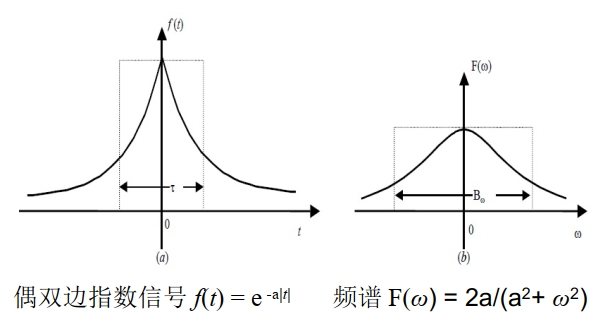
\includegraphics[width = 0.6\linewidth]{chap2/img/equivalent-bandwidth-and-pulse-width.png}
        \caption{等效脉宽与等效带宽}
        \label{fig:equivalent-bandwidth-and-pulse-width}
    \end{figure}
\end{example}

\begin{note}
    有时不特别区分频率和角频率,对 $B_f$ 与 $B_\omega$ 也不做特别区分。
\end{note}

\subsubsection{FT 的时移特性}

\begin{property}
    设信号 $f(t)$ 的 FT 为 $F(\omega)$,则有
    \begin{align*}
        \mathcal{F}[f(t - t_0)] = F(\omega)\mathe^{-\mathi\omega t_0}.
    \end{align*}
    时域延时,频域则是\bd{相位变化},不影响幅度谱,只在相位谱上叠加一个线性相位。

    与尺度变换结合,可以得到 $f(at - t_0)$ 的 FT 为
    \begin{align*}
        \mathcal{F}[f(at - t_0)] = \frac{1}{|a|}F\left(\frac{\omega}{a}\right)\mathe^{-\mathi\omega t_0}.
    \end{align*}
    因为 $f(at - t_0)$ 可以看做是 $f(t)$ 先向右平移 $t_0 / a$ 个单位,再压扩 $a$ 倍得到的。
\end{property}

\begin{remark}
    人耳通过相位信息差异,可以判定声音的远近变化。
    但声音信号的相位变化不影响内容上的理解。
\end{remark}

\subsubsection{FT 的频移特性}

\begin{property}
    设信号 $f(t)$ 的 FT 为 $F(\omega)$,则有
    \begin{align*}
        \mathcal{F}[\mathe^{\mathi\omega_0 t}f(t)] = F(\omega - \omega_0).
    \end{align*}
    这说明,频域上的频移会导致时域上的相位变化。相位增加,频谱右移。

    与尺度变换结合,可以得到当 $a \neq 0$ 时,$\frac{1}{|a|}\mathe^{\mathi\omega_0 t/a}f(t/a)$ 的 FT 为
    \begin{align*}
        \mathcal{F}\left[\frac{1}{|a|}\mathe^{\mathi\omega_0 t/a}f(t/a)\right] = F(a\omega - \omega_0).
    \end{align*}
\end{property}

\begin{remark}
    理论上,时域信号乘以一个复指数信号,原信号的频谱将被搬移到复指数信号的频率处。
    实际应用中,利用欧拉公式,通过乘以\bd{正弦或余弦信号},也可以达到频谱搬移的目的。

    本质上,这都是因为 $\mathcal{F}[\mathe^{\mathi \omega_0 t}] = 2\pi\delta(\omega - \omega_0)$。
\end{remark}

\begin{note}
    有关 FT 的\bd{波形运算}的小结如下,设 $f(t) \iff F(\omega)$:
    \begin{itemize}
        \item 反褶:$f(-t) \iff F(-\omega)$。
        \item 平移:$f(t - t_0) \iff F(\omega)\mathe^{-\mathi\omega t_0}, F(\omega - \omega_0) \iff f(t)\mathe^{\mathi\omega_0 t}$。
    \end{itemize}
    即,时域延时,幅度谱不变;频谱搬移,通过在时域乘以复指数信号实现。
\end{note}

\subsubsection{FT 的微分与积分特性}

\begin{note}
    % TODO:证明
    以下特性的证明都是\bd{错误的},还在完善中。
\end{note}

\begin{property}[微分特性]
    设 $f(t)$ 是一个信号,其 FT 为 $F(\omega)$,则有
    \begin{itemize}
        \item (时域微分)
            \begin{align*}
                \mathcal{F}\left[\frac{\D}{\D{t}}f(t)\right] = \mathi \omega F(\omega)
            \end{align*}
        \item (频域微分)
            \begin{align*}
                \mathcal{F}^{-1}\left[\frac{\D}{\D{t}}F(\omega)\right] = -\mathi t f(t)
            \end{align*}
    \end{itemize}
\end{property}

\begin{proof}
    由于
    \begin{align*}
        f(t) = \frac{1}{2\pi}\int_{-\infty}^{+\infty}F(\omega)\mathe^{\mathi \omega t}\D{\omega},
    \end{align*}
    对 $f(t)$ 求导,有
    \begin{align*}
        \dfrac{\D}{\D{t}}f(t) & = \dfrac{\D}{\D{t}}\left[\frac{1}{2\pi}\int_{-\infty}^{+\infty}F(\omega)\mathe^{\mathi \omega t}\D{\omega}\right] \\
        & = \mathi \omega \frac{1}{2\pi}\int_{-\infty}^{+\infty}F(\omega)\mathe^{\mathi \omega t}\D{\omega} \\
        & = \mathi \omega f(t).
    \end{align*}
    因此
    \begin{align*}
        \mathcal{F}\left[\frac{\D}{\D{t}}f(t)\right] = \mathcal{F}[\mathi \omega f(t)] = \mathi \omega F(\omega).
    \end{align*}
    同理,
    \begin{align*}
        F(\omega) = \int_{-\infty}^{+\infty}f(t)\mathe^{-\mathi \omega t}\D{t},
    \end{align*}
    对 $F(\omega)$ 求导,有
    \begin{align*}
        \dfrac{\D}{\D{\omega}}F(\omega) & = \dfrac{\D}{\D{\omega}}\left[\int_{-\infty}^{+\infty}f(t)\mathe^{-\mathi \omega t}\D{t}\right] \\
        & = -\mathi t \int_{-\infty}^{+\infty}f(t)\mathe^{-\mathi \omega t}\D{t} \\
        & = -\mathi t F(\omega).
    \end{align*}
    因此
    \begin{align*}
        \mathcal{F}^{-1}\left[\frac{\D}{\D{t}}F(\omega)\right] = \mathcal{F}^{-1}[-\mathi t F(\omega)] = -\mathi t f(t).
    \end{align*}
    命题得证。
\end{proof}

\begin{property}[积分特性]
    设 $f(t)$ 是一个信号,其 FT 为 $F(\omega)$,则有
    \begin{itemize}
        \item (时域积分)
            \begin{align*}
                \mathcal{F}\left[\int_{-\infty}^{t}f(\tau)\D{\tau}\right] = \frac{F(\omega)}{\mathi\omega} + \pi F(0)\delta(\omega)
            \end{align*}
        \item (频域积分)
            \begin{align*}
                \mathcal{F}^{-1}\left[\int_{-\infty}^{\omega}F(\lambda)\D{\lambda}\right] = \frac{f(t)}{-\mathi t} + \pi f(0)\delta(t)
            \end{align*}
    \end{itemize}
\end{property}

\begin{proof}
    记 $g(t) = \int_{-\infty}^{t}f(\tau)\D{\tau} - F(0)$,由于
    \begin{align*}
        F(0) = \int_{-\infty}^{+\infty}f(t)\D{t},
    \end{align*}
    则 $\lim_{t \to +\infty}g(t) = 0$,且$\frac{\D}{\D{t}}g(t) = f(t)$。
    由微分性质得
    \begin{align*}
        F(\omega) = \mathcal{F}[f(t)] = \mathcal{F}[\frac{\D}{\D{t}}g(t)] = \mathi \omega \mathcal{F}[g(t)],
    \end{align*}
    也就是说,
    \begin{align*}
        F(\omega) & = \mathi \omega \mathcal{F}\left[\int_{-\infty}^{t}f(\tau)\D{\tau} - F(0)\right] \\
        & = \mathi \omega \left(\mathcal{F}\left[\int_{-\infty}^{t}f(\tau)\D{\tau}\right] - \mathcal{F}[F(0)]\right) \\
        & = \mathi \omega \left(\mathcal{F}\left[\int_{-\infty}^{t}f(\tau)\D{\tau}\right] - 2\pi F(0)\delta(\omega)\right).
    \end{align*}
    因此
    \begin{align*}
        \mathcal{F}\left[\int_{-\infty}^{t}f(\tau)\D{\tau}\right] = \frac{F(\omega)}{\mathi\omega} + \pi F(0)\delta(\omega).
    \end{align*}
    同理,记 $G(\omega) = \int_{-\infty}^{\omega}F(\lambda)\D{\lambda} - 2\pi f(0)$,由于
    \begin{align*}
        f(0) = \frac{1}{2\pi}\int_{-\infty}^{+\infty}F(\omega)\D{\omega},
    \end{align*}
    则 $\lim_{\omega \to +\infty}G(\omega) = 0$,且$\frac{\D}{\D{\omega}}G(\omega) = F(\omega)$。由微分性质得
    \begin{align*}
        f(t) = \mathcal{F}^{-1}[F(\omega)] = \mathcal{F}^{-1}[\frac{\D}{\D{\omega}}G(\omega)] = -\mathi t \mathcal{F}^{-1}[G(\omega)],
    \end{align*}
    也就是说,
    \begin{align*}
        f(t) & = -\mathi t \left(\mathcal{F}^{-1}\left[\int_{-\infty}^{\omega}F(\lambda)\D{\lambda}\right] - \mathcal{F}^{-1}[2\pi f(0)]\right) \\
        & = -\mathi t \left(\mathcal{F}^{-1}\left[\int_{-\infty}^{\omega}F(\lambda)\D{\lambda}\right] - 2\pi f(0)\delta(t)\right).
    \end{align*}
    因此
    \begin{align*}
        \mathcal{F}^{-1}\left[\int_{-\infty}^{\omega}F(\lambda)\D{\lambda}\right] = \frac{f(t)}{-\mathi t} + \pi f(0)\delta(t).
    \end{align*}
    命题得证。
\end{proof}

\subsubsection{FT 的卷积特性}

\begin{theorem}[时域卷积定理]
    设有信号 $f_1(t)$ 和 $f_2(t)$,则有
    \begin{align*}
        \mathcal{F}[f_1(t) * f_2(t)] = \mathcal{F}[f_1(t)] \cdot \mathcal{F}[f_2(t)].
    \end{align*}
\end{theorem}

\begin{proof}
    根据卷积的定义,有
    \begin{align*}
        f_1(t) * f_2(t) = \int_{-\infty}^{+\infty} f_1(\tau)f_2(t - \tau)\D{\tau}.
    \end{align*}
    对上式两边同时求 FT,有
    \begin{align*}
        \mathcal{F}[f_1(t) * f_2(t)] & = \int_{-\infty}^{+\infty} \left[\int_{-\infty}^{+\infty} f_1(\tau)f_2(t - \tau)\D{\tau}\right]\mathe^{-\mathi\omega t}\D{t} \\
        & = \int_{-\infty}^{+\infty} f_1(\tau)\left[\int_{-\infty}^{+\infty} f_2(t - \tau)\mathe^{-\mathi\omega t}\D{t}\right]\D{\tau} \\
        & = \int_{-\infty}^{+\infty} f_1(\tau)\left[\int_{-\infty}^{+\infty} f_2(t)\mathe^{-\mathi\omega(t + \tau)}\D{t}\right]\D{\tau} \\
        & = \int_{-\infty}^{+\infty} f_1(\tau)\left[\int_{-\infty}^{+\infty} f_2(t)\mathe^{-\mathi\omega t}\D{t}\right]\mathe^{-\mathi\omega\tau}\D{\tau} \\
        & = \left[\int_{-\infty}^{+\infty} f_1(\tau)\mathe^{-\mathi\omega\tau}\D{\tau}\right]\left[\int_{-\infty}^{+\infty} f_2(t)\mathe^{-\mathi\omega t}\D{t}\right] \\
        & = \mathcal{F}[f_1(t)] \cdot \mathcal{F}[f_2(t)].
    \end{align*}
    命题得证。
\end{proof}

\begin{theorem}[频域卷积定理]
    设有信号 $f_1(t)$ 和 $f_2(t)$,则有
    \begin{align*}
        \mathcal{F}[f_1(t) \cdot f_2(t)] = \dfrac{1}{2\pi}\mathcal{F}[f_1(t)] * \mathcal{F}[f_2(t)].
    \end{align*}
\end{theorem}

\begin{proof}
    不妨设 $f_1(t)$ 和 $f_2(t)$ 的 FT 分别为 $F_1(\omega)$ 和 $F_2(\omega)$。
    根据卷积的定义,有
    \begin{align*}
        F_1(\omega) * F_2(\omega) = \int_{-\infty}^{+\infty} F_1(\eta)F_2(\omega - \eta)\D{\eta}.
    \end{align*}
    对上式两边同时求 IFT,有
    \begin{align*}
        \mathcal{F}^{-1}[F_1(\omega) * F_2(\omega)] & = \frac{1}{2\pi}\int_{-\infty}^{+\infty} \left[\int_{-\infty}^{+\infty} F_1(\eta)F_2(\omega - \eta)\D{\eta}\right]\mathe^{\mathi\omega t}\D{\omega} \\
        & = \frac{1}{2\pi}\int_{-\infty}^{+\infty} F_1(\eta)\left[\int_{-\infty}^{+\infty} F_2(\omega - \eta)\mathe^{\mathi\omega t}\D{\omega}\right]\D{\eta} \\
        & = \frac{1}{2\pi}\int_{-\infty}^{+\infty} F_1(\eta)\left[\int_{-\infty}^{+\infty} F_2(\omega)\mathe^{\mathi(\omega + \eta)t}\D{\omega}\right]\D{\eta} \\
        & = \frac{1}{2\pi}\int_{-\infty}^{+\infty} F_1(\eta)\left[\int_{-\infty}^{+\infty} F_2(\omega)\mathe^{\mathi\omega t}\D{\omega}\right]\mathe^{\mathi\eta t}\D{\eta} \\
        & = 2\pi\cdot\left[\frac{1}{2\pi}\int_{-\infty}^{+\infty} F_1(\eta)\mathe^{\mathi\eta t}\D{\eta}\right]\left[\frac{1}{2\pi}\int_{-\infty}^{+\infty} F_2(\omega)\mathe^{\mathi\omega t}\D{\omega}\right] \\
        & = 2\pi \mathcal{F}^{-1}[F_1(\omega)] \cdot \mathcal{F}^{-1}[F_2(\omega)] \\
        & = 2\pi f_1(t) \cdot f_2(t).
    \end{align*}
    对上式两边同时求 FT,有
    \begin{align*}
        F_1(\omega) * F_2(\omega) = \mathcal{F}[2\pi f_1(t) \cdot f_2(t)],
    \end{align*}
    即
    \begin{align*}
        \mathcal{F}[f_1(t) \cdot f_2(t)] = \frac{1}{2\pi}F_1(\omega) * F_2(\omega).
    \end{align*}
    命题得证。
\end{proof}

\begin{example}
    若信号在截取时,是使用``与矩形脉冲函数''相乘来实现的,
    即,设有信号 $f_1(t)$ 和 $f_2(t) = G_{\tau}(t)$,则
    \begin{align*}
        \mathcal{F}[f_1(t) \cdot f_2(t)] = \frac{1}{2\pi}\mathcal{F}[f_1(t)] * \mathcal{F}[f_2(t)] = \frac{1}{2\pi}\mathcal{F}[f_1(t)] * \tau\sa\left(\frac{\tau\omega}{2}\right).
    \end{align*}
\end{example}

\begin{remark}
    但实际情况下不存在理想的矩形信号。矩形信号边缘的跳变,将引起原信号的频谱产生畸变。
\end{remark}

\subsubsection{FT 时域上的相关性定理}

\begin{theorem}
    设信号 $f_1(t)$ 和 $f_2(t)$ 的 FT 分别为 $F_1(\omega)$ 和 $F_2(\omega)$,则有
    \begin{align*}
        \mathcal{F}[R_{f_1, f_2}(t)] = \mathcal{F}[f_1(t)] \cdot \mathcal{F}^*[f_2(t)].
    \end{align*}
    特别地,若 $f_2(t)$ 为实偶函数,则 $\mathcal{F}[R_{f_1, f_2}(t)] = F_1(\omega)F_2(\omega)$。

    自相关的 FT 定义为
    \begin{align*}
        \mathcal{F}[R_f(t)] = \mathcal{F}[f(t)] \cdot \mathcal{F}^*[f(t)] = \|\mathcal{F}[f(t)]\|^2.
    \end{align*}
    这说明信号自相关函数与其幅度谱平方,是一对傅里叶变换对。
\end{theorem}

\begin{proof}
    由相关运算和 FT 的时域卷积定理,以及 FT 的共轭性质,有
    \begin{align*}
        \mathcal{F}[R_{f_1, f_2}(t)] & = \mathcal{F}[f_1(t) * f_2^*(-t)] \\
        & = \mathcal{F}[f_1(t)] \cdot \mathcal{F}[f_2^*(-t)] \\
        & = \mathcal{F}[f_1(t)] \cdot \mathcal{F}^*[f_2(t)].
    \end{align*}
    命题得证。
\end{proof}

\subsubsection{FT 的帕斯瓦尔定理}

\begin{theorem}
    设 $f(t)$ 是一个时域上的信号,其傅里叶变换为 $F(\omega)$,则有
    \begin{align*}
        \int_{-\infty}^{+\infty} \|f(t)\|^2 \D{t}
        = \frac{1}{2\pi}\int_{-\infty}^{+\infty} \|F(\omega)\|^2 \D{\omega}
        = \int_{-\infty}^{+\infty}\|F(2\pi f)\|^2 \D{f}.
    \end{align*}
    这说明,信号的能量在时域和频域上是守恒的。
\end{theorem}
